\section{Détection de la plaque}
Pour détecter une plaque sur une image, nous avons choisi l’\textbf{approche par apprentissage automatique}. À cet effet, nous avons entraîné un modèle Deep Learning de détection d’objets en utilisant l’architecture YOLOv4 Tiny. Le choix de cette architecture s’explique par ses performances qui sont clairement définies dans le tableau \ref{table:yolo}. D’autre part, cette architecture est la plus adaptée pour les appareils mobiles et systèmes embarqués où nous avons déployé le modèle de détection à cause de sa taille réduite qui la rend plus rapide. Décrivons maintenant chaque étape que nous avons suivie pour avoir le modèle.
    \subsection{Acquisition des données}
    L’entraînement d’un modèle de Deep Learning nécessite une masse importante de données. Pour la détection des plaques, nous avons collecté les images de véhicules sur la plateforme \textbf{Open Images de Google}. Open Images est une base de données en ligne d'environ 9 millions d'images annotées \cite{oid6}. Sur cette plateforme, nous avons pu  avoir \textbf{5890 images avec les annotations sous format YOLO d’une taille d’environ 2 Go}. Les annotations sont des fichiers texte contenant les coordonnées des cadres de délimitation des plaques. 
    \begin{figure}[H]
        \centering
        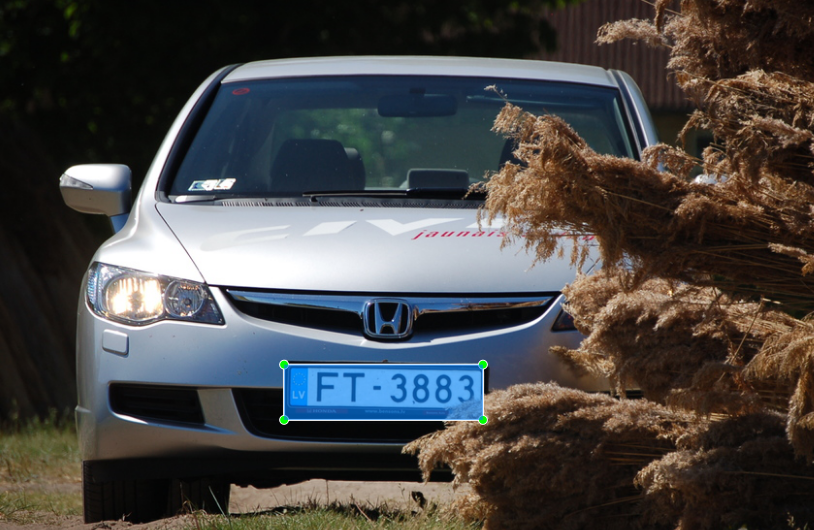
\includegraphics[scale=0.3]{imageDataset}
        \caption{Exemple d'images collectées sur Open Images}
    \end{figure}
    Après une analyse des données collectées, voici quelques unes de ses caractéristiques:
    \begin{table}[H]
        \centering
        \begin{tabular}{|l|l|}
            \hline
            \rowcolor{Gray}
            \textbf{Caractéristiques} & \textbf{Valeur} \\ \hline
            Largeur maximale des images & \textbf{2672px} \\ \hline
            Hauteur maximale des images & \textbf{4000px} \\ \hline
            Largeur minimale des images & \textbf{141px} \\ \hline
            Hauteur minimale des images & \textbf{225px} \\ \hline
            Nombre maximal d'annotations sur une image & \textbf{26} \\ \hline
            Moyenne du nombre d'annotations par image & \textbf{1.43} \\ \hline
            Nombres d'images dupliquées & \textbf{134} \\ \hline
        \end{tabular}
        \caption{Analyse de la collection des données de véhicules}
    \end{table}
    \subsection{Nettoyage et préparation}
    Avant d’utiliser les données collectées, il est important de les vérifier et corriger les anomalies afin d’éviter des mauvaises performances du modèle. À l’aide de l’outil d’annotations \textbf{LabelImg}, nous avons vérifié si toutes les images que nous avions chargées étaient bien annotées. Dans certains cas où les cadres de délimitation des plaques étaient mal placés, il fallait les repositionner. D’autre part, nous avons remarqué comme l’indique le tableau précédent que 134 images ont été dupliquées. À l’aide d’un script écrit en Python, nous avons supprimé toutes ces duplications. Nous obtenons finalement une base de données de 5756 images distinctes et correctement annotées. Par ailleurs, grâce à la plateforme en ligne Roboflow, nous avons effectué quelques opérations de prétraitement sur l’ensemble des images. Ces opérations permettent d’une part de réduire le temps d’entraînement du modèle et d’autre part d'améliorer la précision du modèle. Parmi ces opérations, on retrouve l’\textbf{auto-orientation} pour standardiser l’ordre des pixels et le \textbf{redimensionnement à 416 x 416} (taille d’entrée du modèle).
    \subsection{Entraînement du modèle}
    Pour l’évaluation de la performance du modèle au cours de l’entraînement, nous avons subdivisé notre base de données en deux grands groupes: \textbf{80\% soit 4604 images pour l’entraînement et 20\% pour le test}. L’entraînement du modèle a été fait sur la plateforme en ligne Google Colab. Elle offre des ressources(puissance de GPU) gratuitement pour entraîner des modèles de Deep Learning. Voici quelques configurations prises en compte:
    \begin{itemize}
        \item \textbf{Type d'exécution: GPU}
        \item \textbf{Utilisation de CUDA Version 11.2}
        \item \textbf{GPU: Tesla T4}
        \item \textbf{Architecture du modèle: YOLO V4}
        \item \textbf{Utilisation de Tensorflow version 2.3.0rc0}
        \item \textbf{Utilisation du \href{https://github.com/roboflow-ai/darknet.git}{repertoire darknet de Roboflow}}
        \item \textbf{Utilisation de fichier de configuration} \href{https://github.com/AlexeyAB/darknet/blob/master/cfg/yolov4-tiny-3l.cfg}{yolov4-tiny\_3l.cfg}: néanmoins, nous avons modifié certains paramètres dans ce fichier.
        \begin{table}[H]
            \centering
            \begin{tabular}{|l|c|}
                \hline
                \rowcolor{Gray}
                \textbf{Paramètres} & \textbf{Nouvelle valeur} \\ \hline
                batch & \textbf{64} \\ \hline
                subdivisions & \textbf{32} \\ \hline
                width & \textbf{416} \\ \hline
                height & \textbf{416} \\ \hline
                max\_batches & \textbf{6000} \\ \hline
                steps & \textbf{4800, 5400} \\ \hline
                classes & \textbf{1} \\ \hline
                filters (couche de convolution avant couche yolo) & \textbf{18} \\ \hline 
            \end{tabular}
            \caption{Quelques paramètres du fichier de configuration YOLO}
        \end{table}
        \item \textbf{Utilisation des poids pré-entraînés YOLO: \href{https://github.com/AlexeyAB/darknet/releases/download/darknet_yolo_v4_pre/yolov4-tiny.conv.29}{yolov4-tiny.conv.29}} 
    \end{itemize}
    L’entraînement a pratiquement pris \textbf{1.5 heures}. Pour analyser la progression de l'entraînement au fil des itérations, le programme d'entraînement nous a généré une courbe représentée dans la figure suivante.
    \begin{figure}[H]
        \centering
        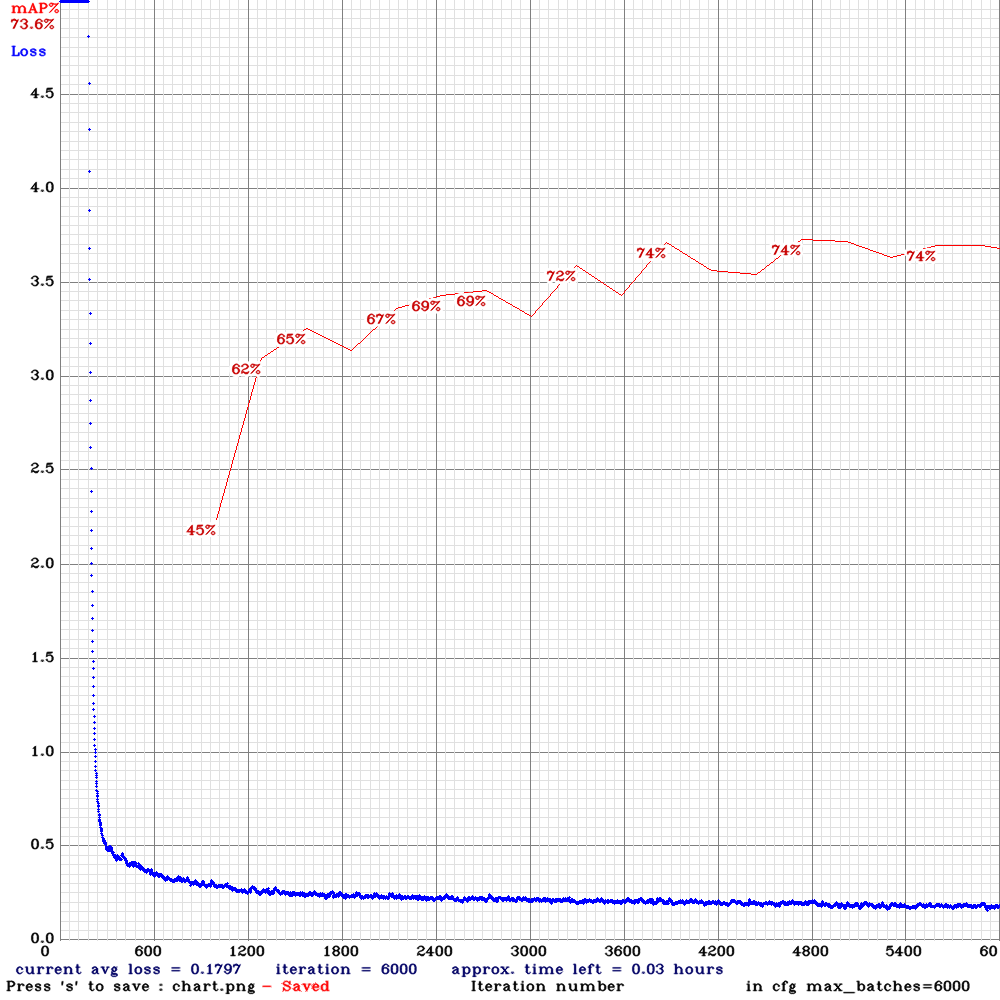
\includegraphics[scale=0.3]{chart1.png}
        \caption{Évolution de la métrique mAP et de l'erreur lors de l'entraînement du modèle de détection de plaques.}
    \end{figure}
    Cette courbe montre l’évolution de la précision du modèle (en rouge) et de l'erreur faite par le modèle sur les données d'entraînement (en bleu) au cours de l’entraînement en fonction du nombre d'itérations. Nous y remarquons bien évidemment la croissance de la précision jusqu'à \textbf{74\%} du modèle et la décroissance de l'erreur jusqu'à pratiquement \textbf{0.2}. Ceci traduit bien le bon déroulement de l'entraînement. À la fin de l'entraînement, un fichier binaire extension \textbf{.weights} contenant les poids du réseaux de neurones entraîné.

    \subsection{Résultats et évaluation}
    Nous avons évalué notre modèle de détection des plaques sur deux types de données: les images contenant des véhicules au Maroc afin d'évaluer la précision du modèle et les vidéos de voitures en circulation afin de mesurer la rapidité du modèle. 
    
    
    Pour le premier type, nous avons collecté des images sur les plateformes comme Kaggle, MSDA Datasets de UM6P et d’autres prises dans la rue. Après avoir réuni ces différentes sources de données, nous avons obtenu une base de données de \textbf{2229 images}. On retrouve en moyenne une plaque par image. Le tableau d’évaluation est décrit comme suit:
    \begin{table}[H]
        \centering
        \begin{tabular}{|l|l|}
            \hline
            \rowcolor{Gray}
            \textbf{Évaluation} & \textbf{Valeur} \\ \hline
            Nombre de plaques correctement détectées (VP) & \textbf{1994} \\ \hline
            Nombre de plaques non détectées (FN) & \textbf{386} \\ \hline
            Nombre de fausses détections (FP) & \textbf{6} \\ \hline
            Précision & \textbf{99,7\%} \\ \hline
            Rappel & \textbf{83,78\%} \\ \hline
        \end{tabular}
        \caption{Évaluation du modèle de détection des plaques marocaines}
    \end{table}
    Puisque la précision et le rappel du modèle sont élevés, on peut dire que le modèle est performant en terme de précision de détection. La figure suivante traduit des exemples de détection faite par le modèle qui a été entraîné.
    \begin{figure}[H]
        \begin{subfigure}{0.3\textwidth}
            \centering
            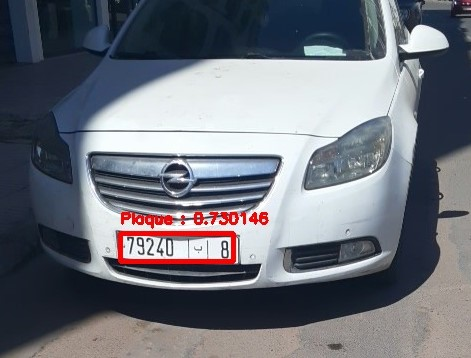
\includegraphics[width=\textwidth]{carMorocco232.jpg}
        \end{subfigure}
        \hfill
        \begin{subfigure}{0.3\textwidth}
            \centering
            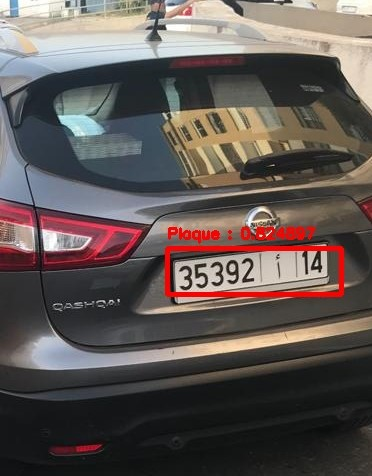
\includegraphics[width=\textwidth]{carMorocco772.jpg}
        \end{subfigure}
        \hfill
        \begin{subfigure}{0.3\textwidth}
            \centering
            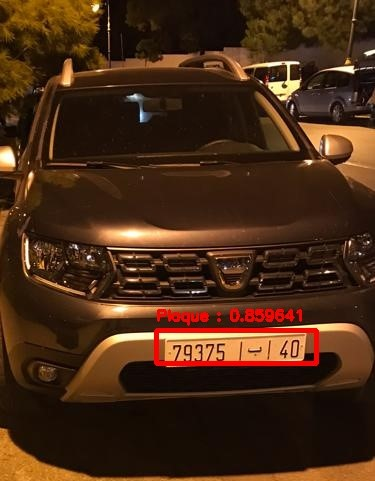
\includegraphics[width=\textwidth]{carMorocco913.jpg}
        \end{subfigure}
        \caption{Exemples de détection de plaques marocaines}
    \end{figure}
    Pour évaluer la rapidité de notre modèle, nous avons lancé le modèle sur des vidéos des véhicules en circulation. Puisque cette rapidité dépend en partie des performances matérielles de la machine sur laquelle le modèle est exécuté, voici ses caractéristiques:
    \begin{table}[H]
        \centering
        \begin{tabular}{|l|l|}
            \hline
            \rowcolor{Gray}
            \textbf{Caractèristiques} & \textbf{Valeur} \\ \hline
            Processeur & \textbf{Intel(R) Core(TM) i5-10210U CPU @ 1.60GHz   2.11 GHz} \\ \hline
            RAM & \textbf{8.00 Go} \\ \hline
            Disque dur SSD & \textbf{237 Go} \\ \hline
            Type de système & \textbf{Système d’exploitation 64 bits, processeur x64} \\ \hline
        \end{tabular}
        \caption{Caractèristiques du PC}
    \end{table}
    En utilisant la librairie de traitement d’images OpenCV, nous avons développé un script en Python qui nous a permis de remarquer qu’avec les performances ci-dessus, notre modèle traite environ \textbf{14 à 18 images par secondes} en d’autres termes \textbf{14-18 FPS}.
    